\section{Half-Sync/Half-Async}

The Half-Sync/Half-Async architectural pattern decouples asynchronous and synchronous service processing in concurrent systems, to simplify programming without unduly reducing performance. The pattern introduces two intercommunicating layers, one for asynchronous and one for synchronous service processing.

\subsection{Kontext}

Ein nebenläufiges (concurrent) System, welches untereinander kommunizierende synchrone und asynchrone Dienste laufen lässt.

\subsection{Problem}

Asynchrones Programmieren erlaubt schnellere Programme, ist aber grundsätzlich schwieriger für den Software Entwickler.
Synchrone Programme sind einfach zu verstehen, u.U aber langsamer (da Signale grundsätzlich asynchron sind).
Um in einem Software-System beides zu erlauben, müssen folgende Punkte eingehalten werden:

\begin{itemize}
	\item Entwickler, welche synchrone Software entwickeln wollen, sollen sich nicht um asynchrone Programmteile kümmern müssen. Dasselbe gilt für Entwickler, welche Asynchrone Programme entwickeln.
	\item Asynchrone und synchrone Services sollen untereinander kommunizieren können, ohne die Performance anderer Programmteile zu beeinträchtigen.
\end{itemize}

\subsection{Lösung}

Das System in zwei Layer aufteilen (sync und async) und dazwischen ein Queue-Layer setzen, damit sie untereinander kommunizieren können.

\subsection{Struktur}

\begin{itemize}
	\item \emph{synchrones Service Layer} betreibt High-Level Dienste. Dienste im Sync. Service Layer laufen in separaten Threads/Prozessen, welche blockieren können
	\item \emph{asynchrones Service Layer} betreibt Low-Level Dienste, welche normalerweise aus einer oder mehreren Externen Event Sourcen entspringen. Dienste in diesem Layer dürfen nicht blockieren, sonst geht die Performance den Bach runter
	\item \emph{queueing Layer} stellt den Mechanismus für die Kommunikation von Diensten in den einzelnen Layers zur Verfügung. Dieser Layer ist zuständig, dass die Dienste benachrichtigt werden, wenn Nachrichten in der Message Queue sind
	\item \emph{external Event Sources} generieren Events, welche vom Async Service Layer empfange und verarbeitet werden. Das sind z.B. Network Interfaces, Disk Controller etc.
\end{itemize}

\begin{figure}[H]
	\centering
	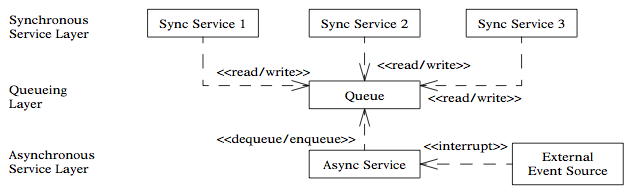
\includegraphics[width=\textwidth]{content/posa2/half-sync-half-async/images/Bildschirmfoto_2013-05-13_um_1.png}
	\caption{component configurator sequencediagram}
\end{figure}

\begin{figure}[H]
	\centering
	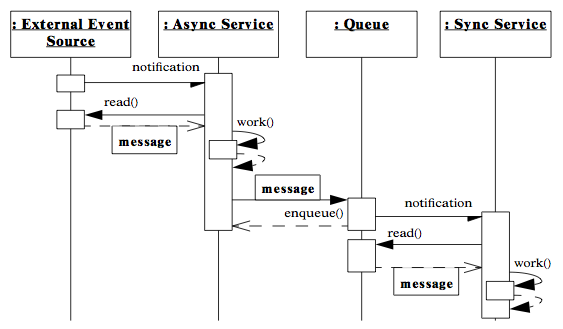
\includegraphics[width=\textwidth]{content/posa2/half-sync-half-async/images/Bildschirmfoto_2013-05-13_um_2.png}
	\caption{component configurator sequencediagram}
\end{figure}

\begin{itemize}
	\item Vereinfachung und Performance: Synchrone Prozesse können einfacher implementiert werden, Asynchrone Prozesse können mit einer hohen Performance entwickelt werden
	\item Separation of Concerns: Synchronizations Policies in jedem Layer sind decoupled
	\item Zentralisierung von Inter-Layer Kommunikation
\end{itemize}

\subsection{Nachteile}

\begin{itemize}
	\item Boundary-Crossing Penalty: Für die Kontextwechsel, die notwendige Synchronisation und das Datenkopieren für die inter-layer Kommunikation (letzteres kann durch gemeinsam genutzte Speicherbereiche verhindert werden)
	\item Komplexität
\end{itemize}


